\section{Tasking System}

The basic unit of execution in \Grappa is a {\em task}. Each hardware core has
a single operating system thread pinned to it. When tasks are ready to
execute, they are mapped to a {\em worker}, which is a user-level thread.
\Grappa keeps a large number of workers per hardware core, which is at the
core of \Grappa's latency tolerance properties. Below we discuss the
implementation of our task management support and then describe how
applications expose parallelism to the \Grappa runtime.

\subsection{Task Support Implementation}

\paragraph{Tasks}
Each task is represented by a function pointer and its arguments, represented
as 32-byte entities: a 64-bit function pointer plus three 64-bit arguments. We
use three arguments because tasks are often generated via a parallel loop
decomposition, in which each task needs three kinds of data. Thus, tasks
include:

\noindent {\it function pointer}, or the addresses of the routine to run ---
we configure the system nodes to disable address randomization, so that
function pointers are valid across process images;

\noindent {\it private argument}, often a loop index; 

\noindent {\it shared argument}, typically data shared amongst a group of
tasks, or the number of loop iterations to be performed by this task;

\noindent {\it synchronization argument}, often used to determine when all
tasks that are part of a loop have finished, in the form of q global pointer
to a synchronization object allocated at the core that spawned a group of
tasks.

While these are the most common uses of the three task arguments, they are
treated as arbitrary 64-bit values in the runtime, and can be used for any
purpose.

\paragraph{Workers}

When a new task is spawned, it is enqueued until it is ready for execution.
Tasks are not allocated any execution resources (a worker) until the scheduler
decides to run them. A worker is simply a collection of status bits and a
stack, allocated at a particular core. There are two types of workers: (1) user worker; and (2) system worker. 

User workers execute application tasks. Once a task is mapped to a worker it
stays with that worker until it completes. System workers execute runtime
management activities such as communication and statistics collection. User
workers and system workers might have different scheduling priorities. System
workers execute periodically and in idle times, to guarantee timely
communication services.

\paragraph{Scheduling} 

During execution, a worker yields control of its core whenever it performs a
long-latency operation, allowing the processor to remain busy while waiting
for the operation to complete. In addition, a programmer can direct scheduling
explicitly via the \Grappa API calls shown in Figure~\ref{fig:scheduling}. To
minimize yield overhead, the \Grappa scheduler operates entirely in user-space
and does little more than store register state of one task and load that of
another.

\begin{figure}[htbp]
  \begin{center}
	\begin{tabular}{l}
    \texttt{\scriptsize yield() } \\
      Yields core to scheduler, enqueuing caller to be \\ scheduled again soon \\
    \texttt{\scriptsize suspend() }  \\
      Yields core to scheduler, enqueuing caller only once \\ another task calls wake \\
    \texttt{\scriptsize wake( task * $t$ ) } \\
      Enqueues some other task $t$ to be scheduled again soon \\
	\end{tabular}
    \begin{minipage}{0.95\columnwidth}
      \caption{\label{fig:scheduling} \Grappa scheduling API } 
    \end{minipage}
  \end{center}
\end{figure}

Each core in a \Grappa system has its own independent scheduler. Each
scheduler has three main responsibilities: servicing system workers that
process communication requests as described in
Section~\ref{sec:communication}; rescheduling workers that have been waiting
on long-latency operations; and assigning ready tasks to worker resources that
have become idle.

Each scheduler has four queues:

\noindent {\it ready worker queue}, a FIFO queue of tasks that are
  matched with workers and are ready to execute;

\noindent {\it private task queue}, a FIFO queue of tasks that must run on this core;

\noindent {\it public task queue},  a LIFO queue of tasks that are
  waiting to be matched with workers. It is a local partition of a shared
  task pool.

\noindent {\it deadline task queue}, a priority queue of tasks that are executed according to task-specific deadline constraints.

Whenever a task yields or suspends, the scheduler makes a decision about what to do next. First, any task in the deadline task queue who's deadline constraint is met is chosen for execution.  This queue manages high priority system tasks, such as periodically servicing communication requests.  Second, the scheduler determines if any workers with running tasks are ready to execute; if so, one is scheduled. Finally, if there are no workers ready to run, but there are tasks waiting to be matched with workers, an idle worker is woken (or a new worker is spawned), matched with a task, and scheduled.

\paragraph{Context switching} \Grappa context switches between workers
non-preemptively. As with other cooperative multithreading systems, we
treat context switches as function calls, saving and restoring only the
callee-saved state as specified in the x86-64 ABI \cite{amd64:abi:2012}. This
involves saving six general-purpose 64-bit registers and the stack
pointer, as well as the 16-bit x87 floating point control word and the
SSE context/status register. Thus, the minimum amount of state a
cooperative context switch routine must save, according to the ABI, is
62~bytes.

\begin{figure}[ht]
    \begin{center}
      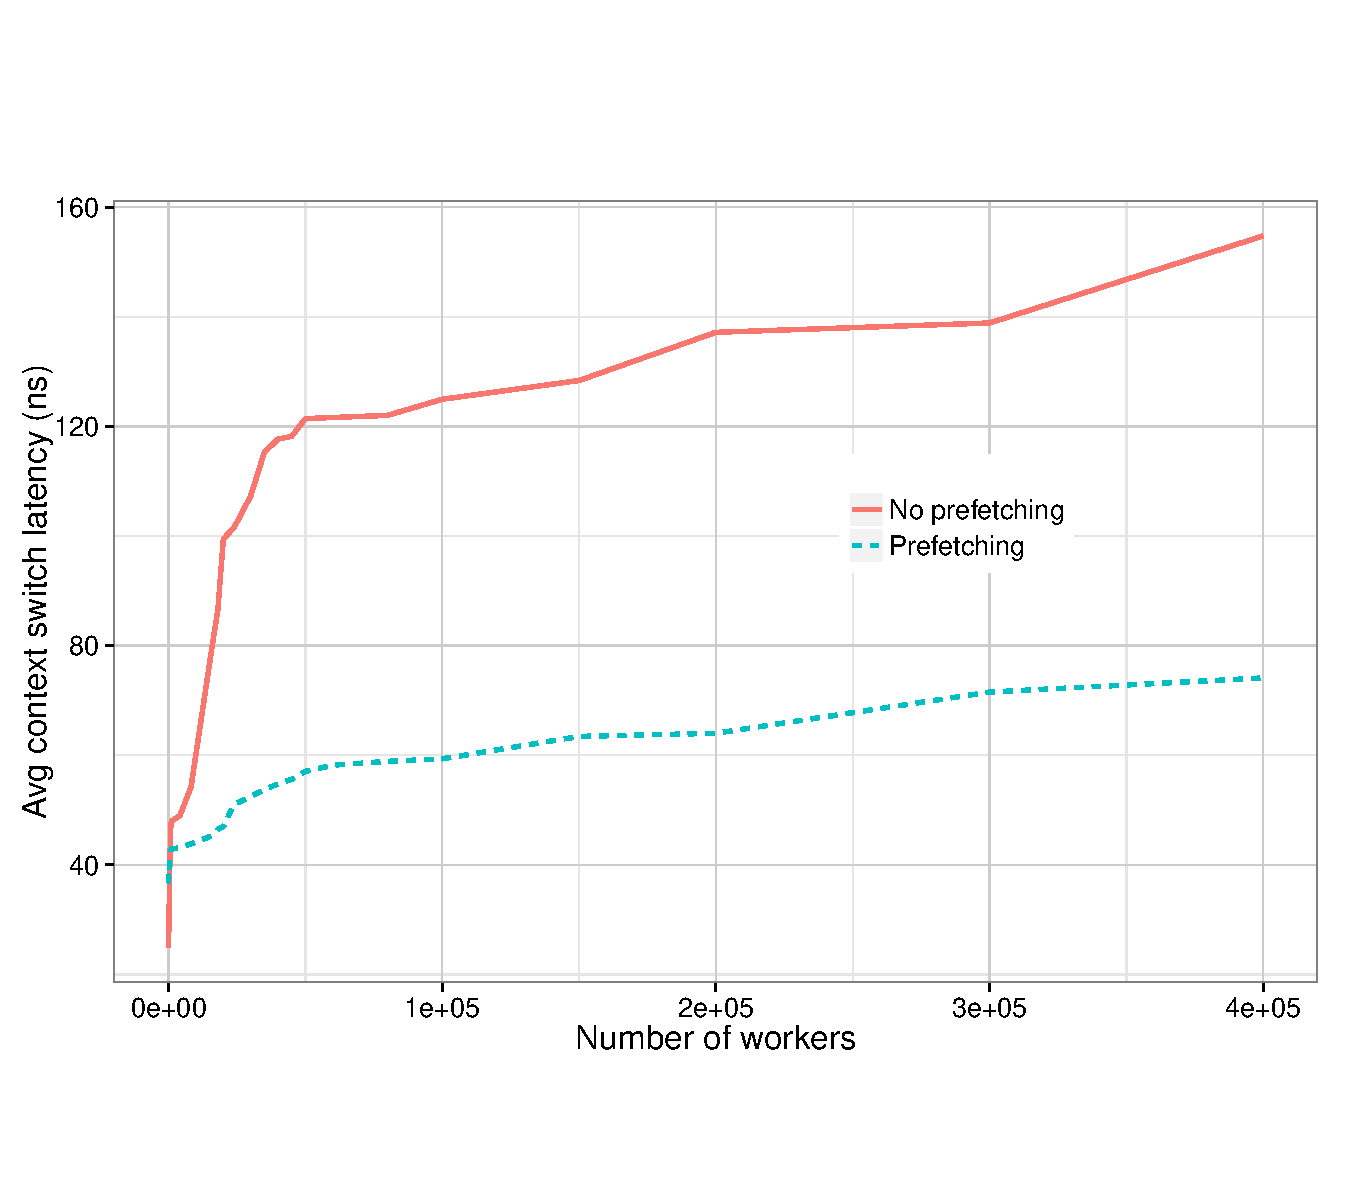
\includegraphics[width=0.5\textwidth]{figs/context_switch_time.pdf}
    \end{center}
    \caption{Average context switch time with 1 and 6 active cores,
        with and without prefetching.}
    \label{fig:context-switch-time}
\end{figure}

\begin{figure}[ht]
    \begin{center}
      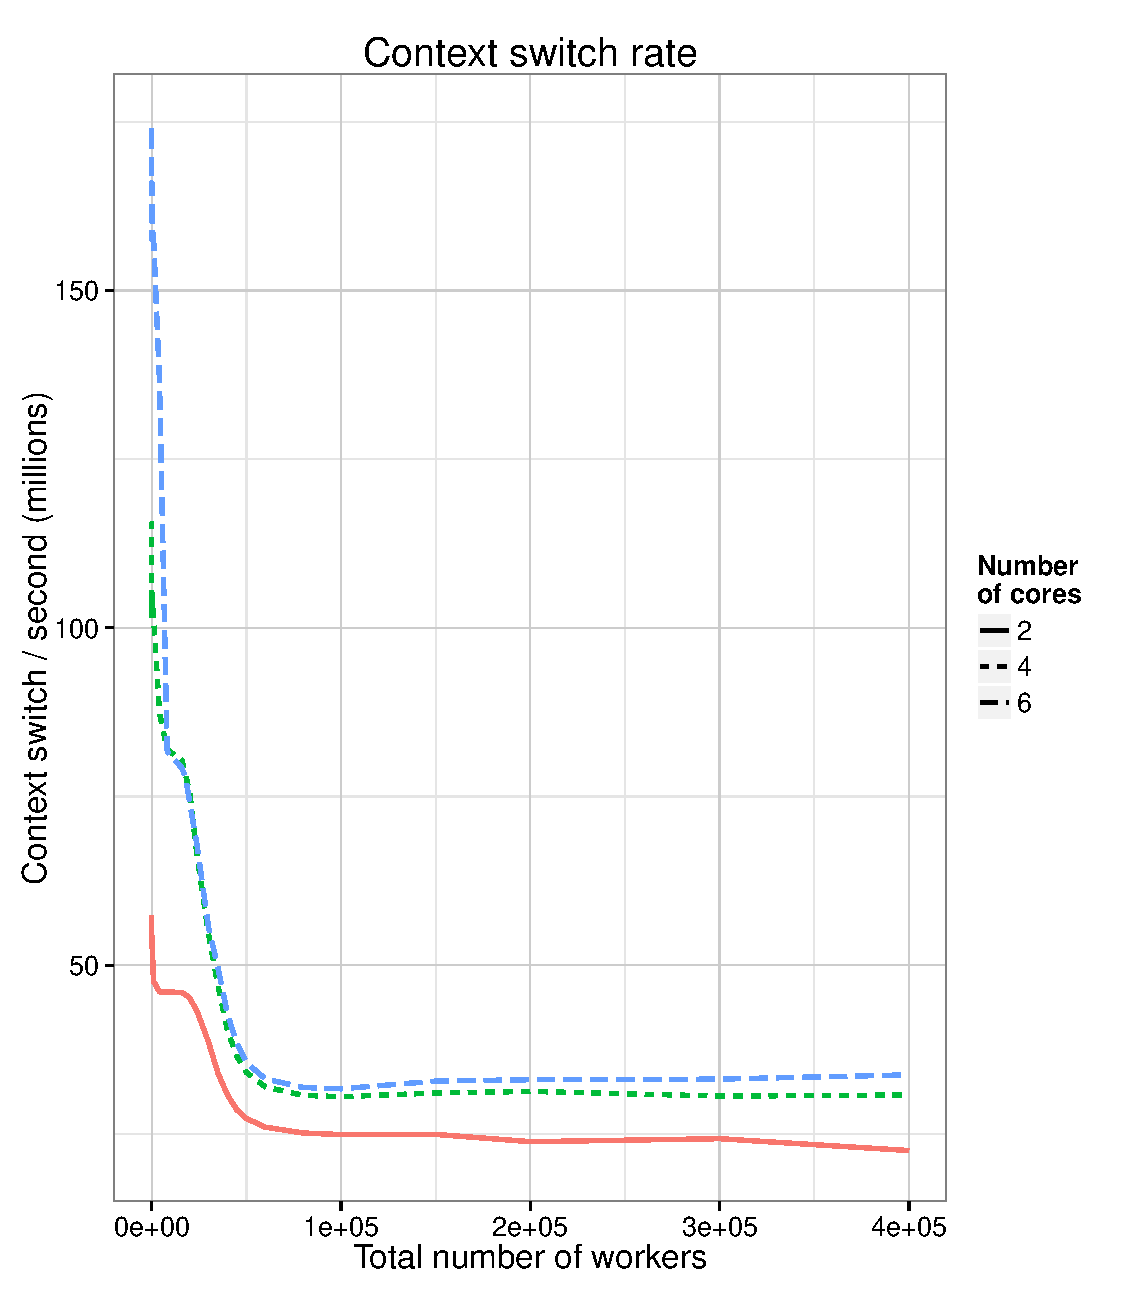
\includegraphics[width=0.5\textwidth]{figs/context_switch_bw.pdf}
    \end{center}
    \caption{Context switch rate with prefetching. Once the total
        size of contexts sufficiently exceeds last-level cache, most
    prefetches go to main memory and the rate becomes limited to the
    off-chip bandwidth.}
    \label{fig:context-switch-time}
\end{figure}

%% No attempt is made to fit them within a single cache line unfortunately :-( Mark
%%% --- importantly, a context is saved in a single 64 byte cache line. 

% Pretty sure this is not true anymore.  Even if it is, it's not important -Mark
%
%Since the compiler sees all calls to the context switch routine, we
%can save even less state. Our context switch routine appears to the
%compiler as inline assembly; we declare all the registers we need
%to save as ``clobbered'' by the inline assembly routine, and the
%compiler will issue its own save and restore code as needed. This allows the
%compiler to avoid saving any registers that are not used, or are used
%for temporary values that are not needed after the context switch.

Since \Grappa keeps a very large number of active workers, their context data will not fit in cache. Therefore, the scheduler has to perform very careful prefetching in order to reduce context switch cost to a minimum. We determined empirically that prefetching the fourth worker in the scheduling order is sufficient. Also determined empirically, we prefetch three cache lines from the stack for each worker.  This makes context switching effectively free of cache misses even to hundreds of thousands of threads.

\TODO{Summary of what to write please expand: Reference above plots. Bandwidth of single socket is
    270Mcacheline/s. Each context is 4 cachelines: 1 for worker struct
    and 3 stack cachelines. We must read and write every context, so 8
    cacheline transfers per context switch. This asymptotically
    approaches 33.75Mcontexts/s as you increase the number of contexts
    (fewer and fewer in L3). Note that only 4+ cores reaches full rate
    because these westmere chips are balanced to not achieve full off-chip bandwidth until 4
    cores--bdmyers}

% When the scheduler chooses a thread to schedule it first looks to see if it must run a periodic task.  If so it choose that.  If not it looks for a ready task.  If none exists it chooses the idle thread.
% 
% If it chooses a task from the ready queue it prefetches the 4'th next thread on the read queue.  Presently 192 bytes of stack are prefetched and 64 bytes of the thread struct itself.
% 
% A periodic task is responsible for looking at the size of the ready queue.  If it is too small more not started tasks are started.
% 

% The context switcher is written entirely in user space.  A context is saved in a single cache line (64 bytes). We prefetch 192 bytes from the stack (which is where the context is saved) in order to prime the stride prefetched on the core and to preload the task state that exists on the stack.


% Fast context switching amongst many tasks is crucial to Grappa for two
% reasons. First, only when the net cost of context switching is dominated by
% the loss incurred by stalling does a latency tolerant approach work to
% increase throughput on computations with intense random access. Random access
% latencies to node local memory are on the order of 100ns. Were the scheduler
% to add more overhead than this, it would actually slow down rather than speed
% up computations that randomly access node local data. Second, because we can
% switch amongst so many tasks without dramatically increasing scheduling
% overhead, Grappa can tolerate system latencies many orders of magnitude
% greater than that of local memory. Network ping latency alone is approximately
% 2us, but our data suggests we can tolerate latencies in the millisecond scale.
% Furthermore, by over-provisioning task parallelism, Grappa promises to provide
% robust throughput that is relatively insensitive to variations in latencies
% within and across our target systems.



\paragraph{Work stealing} 
When the scheduler finds no work to assign to its workers, it commences to
steal tasks from other cores using an asynchronous \texttt{call\_on} active
message. It chooses a victim at random until it finds one with a non-zero
amount of work in its public task queue. The scheduler steals half of the
tasks it finds at the victim. Work stealing is particularly interesting in
\Grappa since performance depends on having many active worker threads on each
core. Even if there are many active threads, if they are all suspended on
long-latency operations, then the core is underutilized. We choose to initiate
one outstanding steal whenever the ready queue is empty there are idle worker
threads.

\comment{Commenting out.  Simon things it doesn't add much I worried about its usefulness too.  -M

\TODO{Anything after this I'm not sure adds to the paper -- if it does, please edit -Simon}
The
core would be fully-utilized if there is always something on the ready
queue. Even if there are many active tasks, if they are all suspended
for long-latency network requests, then the core is underutilized. So,
there is a choice: should the core use some of this idle time to perform
work stealing or should it just wait as it is possible that local tasks
will create more work. We choose to have a core initiate a steal when
all of the following conditions hold: no workers are ready to run, the
unstarted task queues are empty, and there are no outstanding steal
requests. Having only one outstanding steal request throttles steals to
prevent flooding the network, but other scalable quieting mechanisms
would be possible, such as a voting
tree\cite{scalableWorkStealingOrCilk98} or lifelines \cite{lifelines}.
Termination detection is not built into the \Grappa task scheduler,
rather, it is considered a programming error for the program to exit
without syncing all tasks.
}




\subsection{Expressing Parallelism}

\Grappa programmers focus on expressing as much parallelism as possible
without concern for where it will execute. \Grappa then chooses where and when
to exploit this parallelism, scheduling as much work as is necessary on each
core to keep it busy in the presence of system latencies and task dependences.

\Grappa provides four methods for expressing parallelism, shown in
Figure~\ref{fig:expressing-parallelism}. First, when the programmer identifies
work that can be done in parallel, the work may be wrapped up in a function
and queued with its arguments for later execution using a \texttt{spawn}.
Second, a programmer can use \texttt{spawn\_on} to spawn a task on a specific
core in the system or at the home core of a particular memory location. Third,
the programmer can invoke a parallel for loop, provided that the trip count is
known at loop entry. The programmer specifies a function pointer along with
start and end indices and an optional threshold to control parallel overhead.
\Grappa does {\em recursive decomposition} of iterations, similar to Cilk's
cilk\_for construct~\cite {cilkforimplementation}, and TBB's {\tt
parallel\_for}~\cite{intel_tbb}. It generates a logarithmically-deep tree of
tasks, stopping to execute the loop body when the number of iterations is
below the required threshold. Fourth, a programmer may want to execute an active message; that is, to run a
small piece of code on a particular core in the system without waiting for
execution resources to be available. For example, custom synchronization
primitives execute this way, as a function executed on the core where the data
lives. \Grappa provides the \texttt{call\_on} call for this purpose.

\begin{figure}[htbp]
  \begin{center}
    \begin{description}\small
    \item[ \texttt{spawn( void (*fp)(args) )} ] \hfill \\
      Creates a new stealable task
    \item[ \texttt{spawn\_on( core, (*fp)(args) )} ] \hfill \\
      Creates a new private task that will run on a specific core 
    \item[ \texttt{parallel\_for( (*fp)(args), start, end )} ] \hfill \\
      Executes iterations of a loop as stealable tasks 
    \item[ \texttt{call\_on( core, (*fp)(args) )} ] \hfill \\ 
      Runs a limited function on a specific core without consuming
      \Grappa execution resources 
    \end{description}
    \begin{minipage}{0.95\columnwidth}
      \caption{\label{fig:expressing-parallelism} \Grappa API: expressing parallelism
      \TODO{update this with latest C++ code from ``api\_examples.cpp''}
      } % \vspace{-4ex}}
    \end{minipage}
    %\vspace{-3ex}
  \end{center}
\end{figure}

